%!TEX root = ../main.tex
\chapter{Introduction} \label{cap: introduction}
Moore's law has been driving technological advancements in integrated circuits for the past five decades, almost doubling density and speed of microprocessor every two years~\cite{Mack11}. Comparable
technological advancements in hard disk drives (HDDs) have been achieved for capacity increase~\cite{NIST} but not for latency reduction. This technological gap has caused performance of HDDs to fall 
far behind compute components, imposing time penalties of tens of thousands of CPU cycles on data access operations.

Nowadays large scale High Performance Computing (HPC) clusters have thousands of compute nodes (CNs), with hundreds of cores each, connected through a low-latency, high-bandwidth network fabric. 
These systems rely on a separate storage cluster to store, manage and retrieve data. Storage clusters in HPC use HDDs to persistently store large dataset, while different technologies, such as Solid State
Drives (SSDs), are frequently employed for metadata, i.e., small descriptive data generated by the storage system that does not carry any additional information from the user perspective but helps 
the storage system itself perform tasks like restricting access to files to a certain group of users, locating file data blocks in storage devices, and so on.
Large storage clusters have thousands of HDDs distributed across tens or even hundreds of I/O nodes (IONs). The hardware resources in the cluster are managed by a distributed Parallel File Systems (PFSs) 
software such as Lustre~\cite{Braam02} or GPFS~\cite{SchmuckH02}. Parallel file systems try to alleviate the performance gap between compute and storage by chopping up large datasets into smaller units of
fixed size, often called stripes, and distribute them among the available I/O nodes. Multiple parallel paths to the data are then provided, effectively aggregating the I/O bandwidth of single storage devices 
and exporting it to the file system clients in compute nodes. 

In order to effectively exploit storage hardware performance, HPC clusters employee deep I/O software stacks, consisting of several libraries. These libraries have been built incrementally on top of
each other to implement new services as well as to overcome performance bottlenecks. %An example is the Message Passing Interface specifications for parallel I/O (or MPI-IO).
Figure~\ref{figure: hpc-io-stack} shows a typical software stack in HPC.

\begin{figure}[!htb]
  \centering
  \includegraphics[width=0.6\textwidth]{chapters/figures/hpc-io-stack}
  \caption{Example of HPC I/O Stack}
  \label{figure: hpc-io-stack}
\end{figure}

As already anticipated, at the bottom of the stack is the \textit{Storage Infrastructure}, represented by vendor specific hardware/software solutions, which aggregate and export data blocks from storage devices. 
The \textit{Parallel File System} software, on top of the Storage Infrastructure, consolidates these blocks into a file interface, frequently POSIX-IO~\cite{POSIX}. The \textit{I/O Forwarding} layer is optionally used 
in some supercomputer designs, such as the IBM Blue Gene systems, to delegate file system access to a limited number of intermediate I/O clients (proxies), with the benefit of reducing the Operating System (OS) 
noise in compute nodes~\cite{AliCIKLLRWS09}. The \textit{I/O Middleware} provides efficient parallel I/O towards the underlying file system, typically using the MPI-IO interface to achieve high performance data access 
as well as consistency. ROMIO\footnote{Implementation of MPI-IO specifications from Argonne National Laboratory included in the MPICH package (\url{http://www.mpich.org})}~\cite{ThakurGL99} is an example of popular I/O 
middleware library used in HPC. Other widely adopted middlewares are the ADaptable I/O System~\cite{CPE:CPE3125} (ADIOS), SIONlib~\cite{sionlib} and Damaris~\cite{DorierACSO12}. However, these middlewares do not provide applications 
with the infrastructure they need to organize and manage their data in a more abstract and efficient manner. Thus, \textit{Scientific I/O Libraries} have been introduced at the top of the stack to bridge the gap between how 
data is represented and organised at the application level (data model) and how it is mapped onto the underlying file system (storage model). Example of popular I/O libraries include the Hierarchical Data Format library 
(HDF5)~\cite{carlosmalt:folk:sc99} and the network Common Data Format (netCDF)~\cite{1592942}.

To further alleviate performance penalties associated to external I/O operations, modern Operating Systems (OS) use file caching. File caching is a viable technique that relies on main memory to stage data
that is frequently accessed from a file, allowing applications requests to be served from fast RAM instead of slow external storage devices. Caching in general relies on the concept of data locality. Data locality
has two different dimensions, a space dimension and a time dimension. The space dimension is frequently exploited by bringing into the cache more data than requested (prefetch), assuming that spatially contiguous
data has a high probability of being accessed in the future, while the time dimension is exploited by keeping in the cache most recent data and discarding oldest data first, assuming that old data has a lower
probability of being accessed in the future. In file caching these heuristics are implemented using readahead and Last Recently Used (LRU) policies respectively.
These trivial heuristics can consistently improve performance of simple read patterns, e.g. sequential patterns, but cannot help much for scientific applications generating complex read patterns. In fact,
for these applications standard caching policies based on data locality can be harmful rather than useful. Fortunately, file systems ofter provide mechanisms that allow programmers to disclose I/O pattern 
knowledge to the lower layers of the I/O stack through a hints API. The cache manager can then exploit this information to effectively guide data prefetching or to disable the readahead algorithm for random 
patterns. Nevertheless, these hints mechanisms are rarely used by programmers, missing the opportunity to extract the full potential from the underlying storage system.

File caching is also useful in the optimization of write patterns using a writeback approach. In practice the cache is used to buffer (or stage) data written to a file. After data has been staged in the cache
control is returned to the application which can thus progress immediately with its work. Data in the cache is not immediately persisted in the storage system, instead it is synchronized (or written back) to 
the file only after a certain interval of time has passed. The length of this interval depends on a number of factors like the amount of available memory in the node, the number of updates generated, and so on.
However, it has been predicted that the concurrency level in compute nodes at Exascale will increase by a factor of 83, going from 12 to 1,000 cpus, while the amount of memory per node will only increase by 
a factor of 33~\cite{ASCAC2010} as shown in Table~\ref{table: hpc-trend}.

\begin{table}[!htb]
    \centering
    \ra{1.5}
    \caption{Potential Exascale Computer Design for 2018 and its relationship to current HPC designs.}
    \newcolumntype{A}{>{\arraybackslash} m{4cm}}
    \newcolumntype{B}{>{\centering\arraybackslash} m{2cm}}
    \newcolumntype{C}{>{\centering\arraybackslash} m{2cm}}
    \newcolumntype{D}{>{\centering\arraybackslash} m{2cm}}
    \begin{tabular}{ABCD}
        \toprule
        & \bf \small 2010 & \bf \small 2018 & \bf \small Factor Change \\
        \midrule
        \small System Peak         & \small 2 Pf/s     & \small 1 Ef/s     & \small 500   \\
        \small Power               & \small 6 MW       & \small 20 MW      & \small 3     \\
        \small System Memory       & \small 0.3 PB     & \small 10 PB      & \small 33    \\
        \small Node Performance    & \small 0.125 Gf/s & \small 10 Tf/s    & \small 80    \\
        \small Node Memory BW      & \small 25 GB/s    & \small 400 GB/s   & \small 16    \\
        \small Node Concurrency    & \small 12 cpus    & \small 1,000 cpus & \small 83    \\
        \small Interconnect BW     & \small 1.5 GB/s   & \small 50 GB/s    & \small 33    \\
        \small System Size (nodes) & \small 20 K nodes & \small 1 M nodes  & \small 50    \\
        \small Total Concurrency   & \small 225 K      & \small 1 B        & \small 4,444 \\
        \small Storage             & \small 15 PB      & \small 300 PB     & \small 20    \\
        \small I/O Bandwidth       & \small 0.2 TB/s   & \small 20 TB/s    & \small 100   \\
        \bottomrule
    \end{tabular}
    \label{table: hpc-trend}
\end{table}

This trend will translate into a reduced memory capacity per core, thus lowering the amount RAM that can be dedicated to the caching of large datasets. The table also shows that while the system peak will 
increase by a factor of 500, the I/O bandwidth will only increase by a factor of 100, worsening the performance gap between compute and I/O. In the last years new Non-Volatile Memory (NMV) technologies 
have started to enter the HPC market. These devices offer the capacity of HDDs but lower access latency at a higher $ \$ \over GB $ cost. The integration of NVM devices in the storage hierarchy represents an open challenge 
and different approaches are possible. System vendors like Seagate and DDN, just to mention a few, have started using NVM devices, mostly flash based Solid State Drives (SSDs), in their products. Seagate's Nytro 
solution~\cite{Nytro} employes SSDs in high performance storage server to accommodate mixed workloads eliminating performance bottlenecks. DDN's Infinite Memory Engine (IME) solution~\cite{IME} integrates SSDs 
into intermediate I/O proxies nodes (Burst Buffers) that can absorb burst of I/O activity from the file system clients, to subsequently transfer the data to the storage servers. Frequently NVM devices are also available 
in compute nodes, effectively providing an additional tier in the storage hierarchy. Unfortunately, this additional tier is not fully integrated in the I/O software stack.

In the depicted scenario the contribution of this work is two fold. In the first part of the thesis we present Mercury~\cite{CongiuGPMSB}, a transparent guided I/O framework able to optimize file I/O patterns in 
scientific applications, allowing users and administrators to control the I/O behavior of their applications without modifying them. Mercury is especially helpful for converting numerous small read requests into 
a few larger requests using a technique called data sieving. The immediate effect of this optimization is the increase of the application perceived I/O bandwidth, a reduction in the number of I/O requests reaching 
the remote back-end storage devices and, ultimately, in the running time of the application. Additionally, we also present a Virtual File System (VFS) modification of the Linux kernel that allows Mercury to forward 
prefetching hints to the Lustre file system.

In the second part of the thesis we present an optimization for parallel write operations that exploits Non-Volatile Memory (NVM) devices in compute nodes. We demonstrate that the usage of NVM devices as additional
persistent cache can speed up parallel write performance to a shared file in MPI-IO.

The reminder of this thesis is organized as follows. Chapter~\ref{chapter: file-cache} reviews file caching infrastructures in the Linux kernel, also giving a detailed description of the interface used by the kernel
to support I/O hints; Chapter~\ref{chapter: io-pat} reviews the state of the art in I/O pattern analysis and data prefetching; Chapter~\ref{chapter: mercury} presents the Mercury middleware design and implementation;
Chapter~\ref{chapter: deeper} reviews parallel I/O in MPI-IO and presents our solution to integrate NVM devices in ROMIO.

%distributed across many I/O nodes (IONs) connected through a Storage Area Network (SAN). All the available storage resources are managed by a Parallel File System (PFS) software. Since data is ultimately
%stored in HDDs and needs to be accessed through the network, the latency of I/O operations is considerably higher than the CPUs cycle time, making I/O very expensive for applications.
%This performance gap is further exacerbated by the fact that many scientific applications perform small non-contiguous accesses to the parallel file system, that result in a large number of Remote Procedure 
%Calls (RPCs) generated by file system clients sent over the network to the I/O nodes, and a corresponding increase in the number of seek operations on the target disks. 
%In this context, file caching is a well known and widely exploited technique that can reduce or even cancel the performance impact of data access from disk based media. File cache implementations
%normally rely on sub-optimal heuristics to manage data replacement and retention. For example, data prefetching is performed by inspecting the application I/O pattern and reading ahead of the current 
%request if the pattern is sequential. This approach exploits the spatial locality of data in the file and allows following I/O requests to be served from the main memory, hiding the cost of a remote access.
%Similarly, when the cache is full oldest data will be evicted to make room for new data. 
%
%To address this problem, the system software of HPC clusters is built with multiple layers stacked on top of each other. These layers were added incrementally over the years to provide new 
%features/optimizations, and to solve existing problems. Unfortunately, since the corresponding software components were not designed and built in an integrated manner, they often 
%duplicate existing functionalities and introduce additional parameters that make the optimal configuration of the system a very difficult task. Figure~\ref{figure: hpc-io-stack} 
%shows a typical layering for the HPC I/O software stack.
%

%%\section{I/O Middleware Layer} \label{sec: io-middleware}
%In this thesis we focus on the I/O middleware layer of the I/O software stack presented in Figure~\ref{figure: hpc-io-stack}. The I/O middleware represents a key component for achieving high performance 
%in HPC since it connects the parallel file system to the high-level I/O libraries (most commonly HDF5 or netCDF). For this reason the I/O middleware is the best place to implement automatic and semi-automatic 
%optimisations. Contextually, guided I/O interfaces can be used as effective mechanism to deliver the requested optimisation messages.
%
%\section{Guided I/O Interfaces} \label{sec: guided-io}
%Generally guided I/O interfaces come in the form of extensions to the standard API of the main software component. Users, as well as other software packages, can exploit these extensions to control the internal 
%behaviour of the component, altering the way the standard API works. Guided I/O APIs are present at different levels in the I/O software stack but are most commonly found in the I/O middleware and the file system 
%components.
%
%\subsection{Guided I/O in MPI-IO} \label{subsec: mpi-io-hints}
%The ROMIO middleware provides guided I/O support through the MPI-IO hints API, specifically designed to control internal ROMIO parameters and trigger different I/O optimisations. MPI-IO hints are packed into a 
%special info object and passed down to the middleware through the MPI file open API. The MPI-IO hints mechanism allows the middleware to convert I/O patterns generated by applications into I/O patterns that are 
%compatible with the characteristics of the underlying file system, thus improving I/O performance. In this way the same MPI file read and write operations can behave differently depending on the hints passed to the 
%middleware when the file was opened. Specifically, if the collective I/O hint is enabled ROMIO will convert every non-contiguous independent write to the file into a smaller number of sequential coordinated writes.
%
%Besides I/O pattern selection, MPI-IO hints can be also used to control the size of the buffers used by ROMIO when performing I/O, to select the stripe size used by the file system to store data across the available 
%I/O servers and even to select the number of I/O servers used to store the file.
%
%\subsection{Guided I/O in Linux File Systems} \label{subsec: posix-advice}
%At the file system level the Linux kernel provides users with the capability to communicate access pattern information to the local file system through the \texttt{posix\_fadvise()}~\cite{AdviseAPI} system call. 
%The file system can use this information to improve page cache efficiency, for example, by prefetching (or releasing) data that will (or will not) be required soon in the future or by disabling read-ahead in the 
%case of random read patterns. %Nevertheless, \texttt{posix\_fadvise()} is barely used in practice and has intrinsic limitations that discourage its employment in real applications.
%
%The two most used PFSs in HEC clusters nowadays, GPFS and Lustre, are both POSIX compliant. However, neither of them supports the POSIX advice mechanism previously described. GPFS compensates for the lack of POSIX 
%advice support through a hints API that users can access by linking their programs against a service library. Hints are passed to GPFS through the \texttt{gpfs\_fcntl()}~\cite{GPFSHINTS} function and can be used to 
%guide prefetching (or releasing) of file blocks in the page pool\footnote{GPFS pinned memory used for file system caching.}. Lustre, on the other hand, does not provide any client side mechanism similar to GPFS hints 
%or POSIX advice.
%
%\section{Opportunities with Non-Volatile Memories} \label{sec: nvm}
%The availability of Solid State Drives (SSDs) and, more generally, Non-Volatile Memory (NVM) devices in the storage hierarchy provides new opportunities for optimisations based on data placement and migration across 
%the different memory tiers of the system. Although HPC compute nodes have access to locally attached SSDs, these are rarely integrated in the I/O software stack. A possible way of integrating the new memory devices 
%in the stack is given by guided I/O interfaces in the I/O middleware component. By using the guided I/O API in the middleware users can control data placement and migration to improve the efficiency of specific I/O patterns.
%
%One practical use case for NVM devices is file caching. File caching can be useful in many different scenarios. Generally, caching can be used to reduce the I/O latency as well as the number of network requests 
%generated by file system clients. More specifically, since the number of NVM devices can scale linearly with the number of compute nodes in the cluster, it can also improve the aggregated I/O bandwidth. Additionally, 
%caching can be useful to improve collective I/O performance. Collective I/O is a parallel I/O technique in which write performance is highly dependent upon the storage system response time and limited by the slowest writer. 
%The storage system response time in conjunction with the need for global synchronisation, required during every round of data exchange and write, severely impacts collective I/O performance. Future Exascale systems will have 
%an increasing number of processor cores, while the number of storage servers will remain relatively small. Therefore, the storage system concurrency level will further increase, worsening the global synchronisation problem.
%
%NVM file caching can alleviate the global synchronisation problem in collective I/O by minimising the I/O time variation across compute nodes and can increase the I/O bandwidth by aggregating together multiple NVM devices on different compute nodes.
%
%\section{Contribution} \label{sec: contribution}
%In the described context our work provides two main contributions. First, we bring the POSIX Advice and GPFS hints APIs together in a unified middleware component called Mercury~\cite{CongiuGPMSB}. Mercury exports a single API and can transparently select the appropriate underlying hints interface depending on the file system backend used to store the data. Additionally, we modify the Virtual File System (VFS) layer in the Linux kernel to enable the \texttt{posix\_fadvise()} system call for Lustre and more generally any network file system. Second, we integrate new NVM devices inside the ROMIO middleware by extending the MPI-IO hints API~\cite{CongiuNSB}. Locally attached SSDs are thus used to boost collective I/O performance in HPC workloads.
%
%\section{Reminder}
%The reminder of this thesis is organised as follow: Chapter~\ref{chapter: guided-io} presents the state of the art on guided I/O interfaces for different software layers of the I/O stack, more specifically for the MPI-IO API, for Linux file systems and for GPFS; Chapter~\ref{chapter: mercury} presents the Mercury middleware which unifies Linux file systems and GPFS hints API under the same software component; finally Chapter~\ref{chapter: deeper} presents MPI-IO cache hints extensions for the ROMIO middleware. 
